\graphicspath{{\currfiledir/images/}}

%----------------------------------------------------------------------------------------
%	Resultados
%----------------------------------------------------------------------------------------
\chapter{Resultados}
Para a execução dos testes, foram selecionados três grafos, sendo um primeiro bastante simples, utilizado para visualização exata dos valores de centralidade para cada caminho mínimo. Os demais dois grafos são modelos da vida real, clube de karatê de Zachary e a rede de jogos de futebol americano. Buscou-se selecionar redes que contivessem número de vértices e arestas distintas, para que fosse possível obter resultados não viciados em relação ao tamanho do grafo sobre os quais seriam executados os testes. Dito isso, as redes selecionadas representam diferentes tipos de redes e possuem quantidades de vértices que variam de 5 a 115. A Tabela~\ref{sec5:tab_grafos_teste} apresenta a descrição das redes nas quais foram executados os testes propostos.

\begin{table}[!htp]
	\centering
	\caption{Detalhamento das redes selecionadas.}
	\label{sec5:tab_grafos_teste}
	\begin{tabular}{|c|c|c|c|c|}
		\hline
		\textbf{Rede} & \textbf{Vértices} & \textbf{Arestas} & \textbf{Tipo}   & \textbf{Classificação} \\ \hline
		Simple        & 5                 & 6                & Não direcionado & Teste                  \\
		Zachary       & 34                & 78               & Não direcionado & Social                 \\
		Football      & 115               & 613              & Não direcionado & Informação             \\ \hline
	\end{tabular}
\end{table}

A Tabela~\ref{sec5:centralidade_grafo_teste} representa os valores de centralidade calculados para o grafo mais simples, Algoritmo~\ref{sec4:funcao_simple_graph_generator}. A ordem apresentada na tabela depende muito do contexto de análise, para este grafo, foi feita a ordenação de tal forma a agrupar ou deixar mais próximos os vértices iguais, por exemplo, as primeiras linhas desta tabela estão ordenadas primeiro com todos os caminhos mínimos que iniciam no vértice 1 e assim por diante.

\begin{table}[!htp]
	\centering
	\caption{Valores de centralidade do grafo simples, Algoritmo~\ref{sec4:funcao_simple_graph_generator}.}
	\label{sec5:centralidade_grafo_teste}
	\resizebox{3.5cm}{!}{
		\begin{tabular}{|c|c|}
			\hline
			\textbf{Path} & \textbf{Centrality}	\\ \hline
			{[}1, 2{]}    & {[}0.050{]}			\\
			{[}1, 3{]}    & {[}0.075{]}			\\
			{[}1, 5{]}    & {[}0.075{]}			\\
			{[}1, 3, 4{]} & {[}0.016{]} 		\\
			{[}2, 1{]}    & {[}0.050{]}			\\
			{[}2, 3{]}    & {[}0.050{]}			\\
			{[}2, 1, 5{]} & {[}0.016{]} 		\\
			{[}2, 3, 4{]} & {[}0.016{]} 		\\
			{[}3, 1{]}    & {[}0.075{]}			\\
			{[}3, 2{]}    & {[}0.050{]}			\\
			{[}3, 4{]}    & {[}0.075{]}			\\
			{[}3, 1, 5{]} & {[}0.016{]}			\\
			{[}5, 1{]}    & {[}0.075{]}			\\
			{[}5, 4{]}    & {[}0.025{]}			\\
			{[}5, 1, 2{]} & {[}0.016{]} 		\\
			{[}5, 1, 3{]} & {[}0.016{]} 		\\
			{[}4, 3{]}    & {[}0.075{]}			\\
			{[}4, 5{]}    & {[}0.025{]}			\\
			{[}4, 3, 1{]} & {[}0.016{]} 		\\
			{[}4, 3, 2{]} & {[}0.016{]} 		\\ \hline
		\end{tabular}
	}
\end{table}

Já para os grafos do clube de karatê de Zachary e da rede de jogos de futebol americano foram apresentados em gráficos, pois suas tabelas são muito extensas. Serão apresentados dois tipos de gráficos, um com os valores de centralidade dos camino mínimos normalizados e outro com os valores de centralidade, não normalizados e na escala logarítmica, dos caminhos mínimos.

O Gráfico~\ref{sec5:short_path_centrality_ex2} e o Gráfico~\ref{sec5:short_path_centrality_ex3} distribuem os valores de centralidade, normalizados, dos caminhos mínimos no eixo $y$, de forma ordenada (crescente), enquanto o eixo $x$ representa apenas os caminhos mínimos em si, ou seja, estão rotulados sequencialmente, pois nesta visualização o percurso exato de cada um dos caminhos mínimos não nos interessa.

\begin{figure}[!htb]
    \centering
    \begin{subfigure}{.5\textwidth}
        \centering
        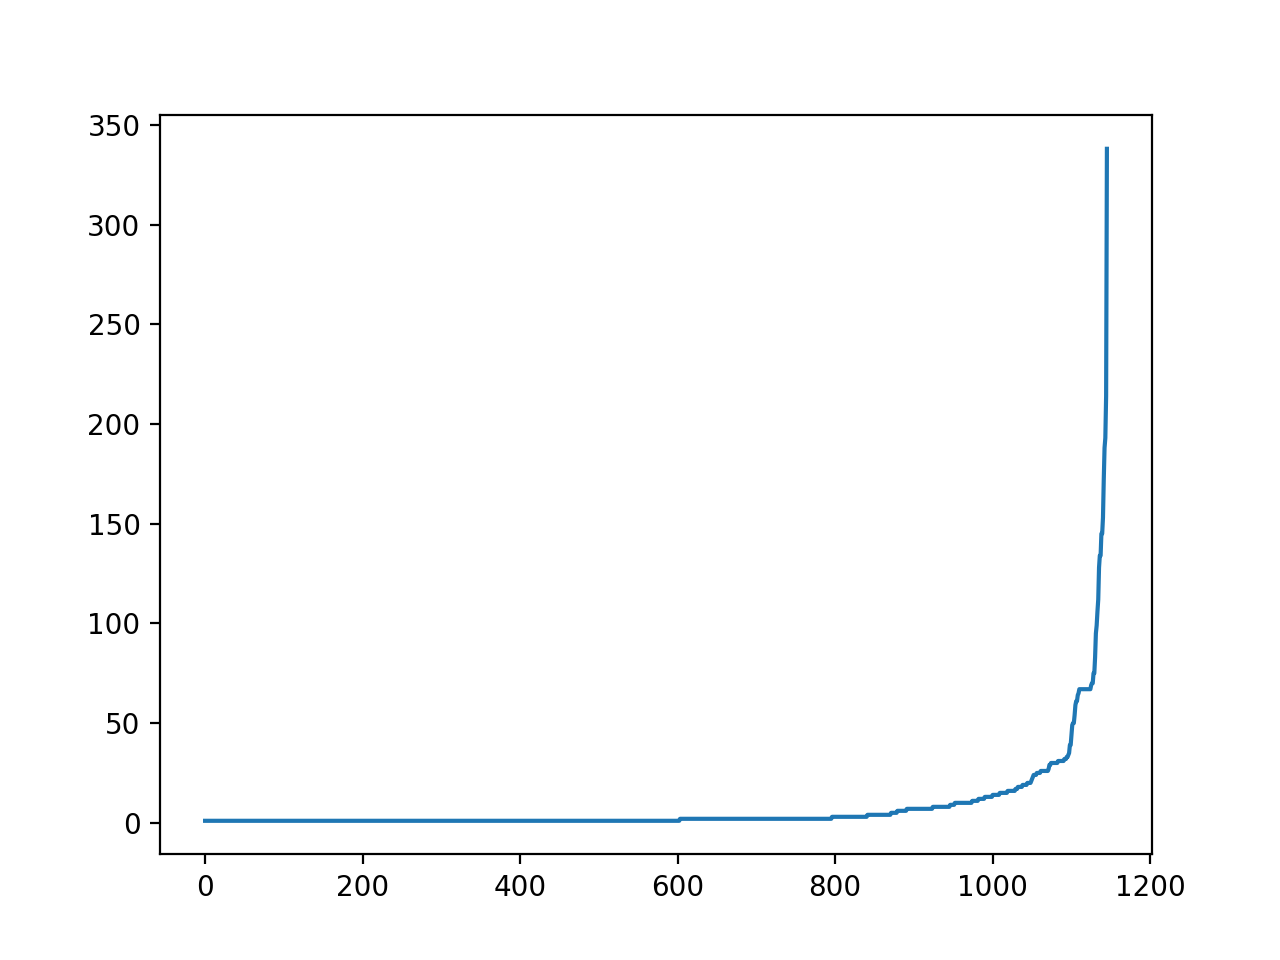
\includegraphics[scale=0.5]{short_path_centrality_ex2.png}
        \caption{Clube de karatê de Zachary.}
        \label{sec5:short_path_centrality_ex2}
    \end{subfigure}%
    \begin{subfigure}{.5\textwidth}
        \centering
        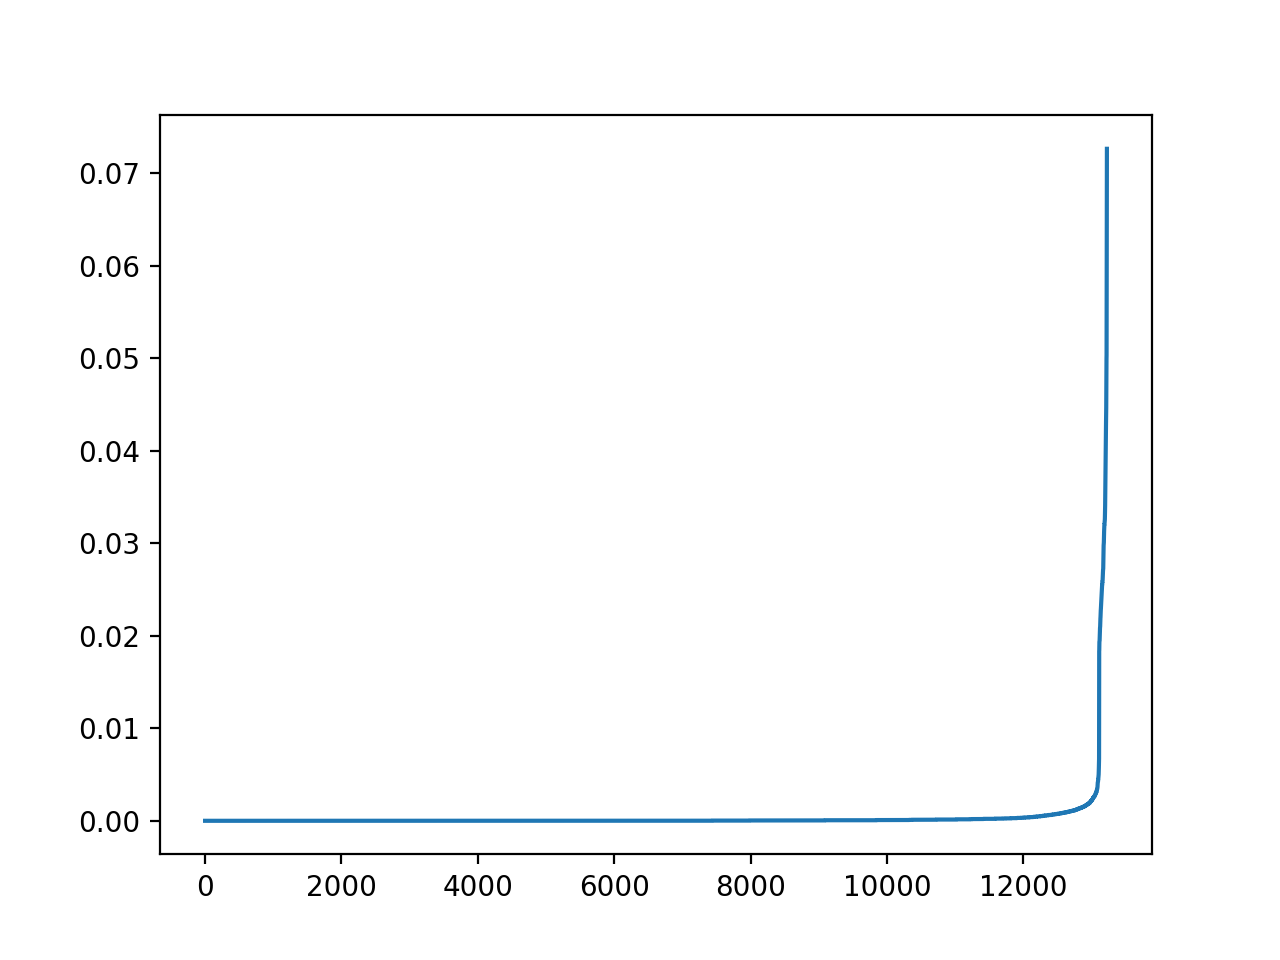
\includegraphics[scale=0.5]{short_path_centrality_ex3.png}
        \caption{Rede de jogos de futebol americano.}
        \label{sec5:short_path_centrality_ex3}
    \end{subfigure}
    \caption{Distribuição dos valores de centralidade, normalizados, dos caminhos mínimos.}
    \label{sec5:grafico_centralidade_normalizados}
\end{figure}

O Gráfico~\ref{sec5:short_path_centrality_ex2_log} e o Gráfico~\ref{sec5:short_path_centrality_ex3_log} distribuem os valores de centralidade, não normalizados e na escala logarítmica, dos caminhos mínimos no eixo $y$, de forma ordenada (crescente).

\begin{figure}[!htb]
    \centering
    \begin{subfigure}{.5\textwidth}
        \centering
        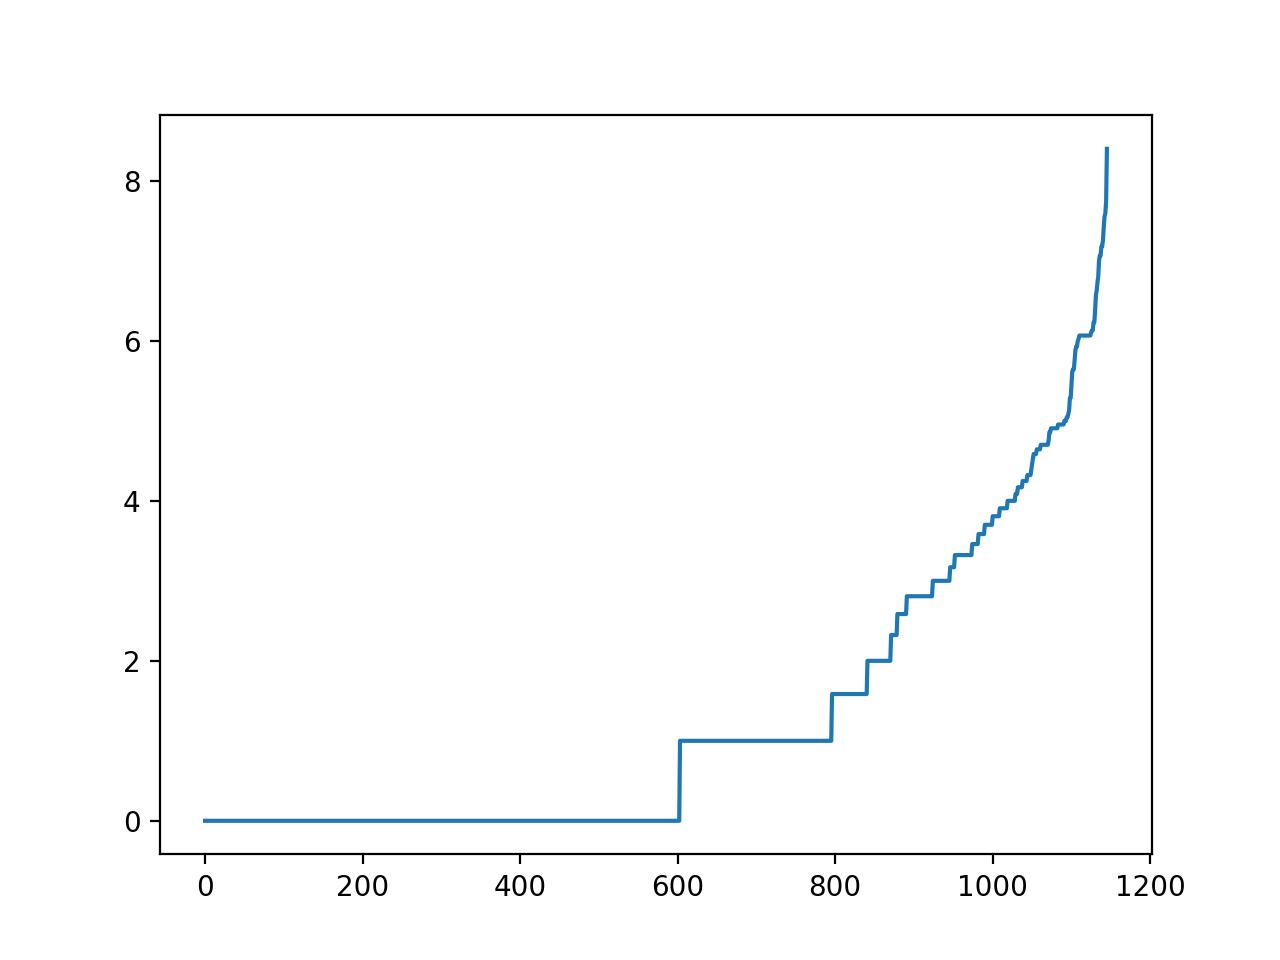
\includegraphics[scale=0.5]{short_path_centrality_ex2_log.png}
        \caption{Clube de karatê de Zachary.}
        \label{sec5:short_path_centrality_ex2_log}
    \end{subfigure}%
    \begin{subfigure}{.5\textwidth}
        \centering
        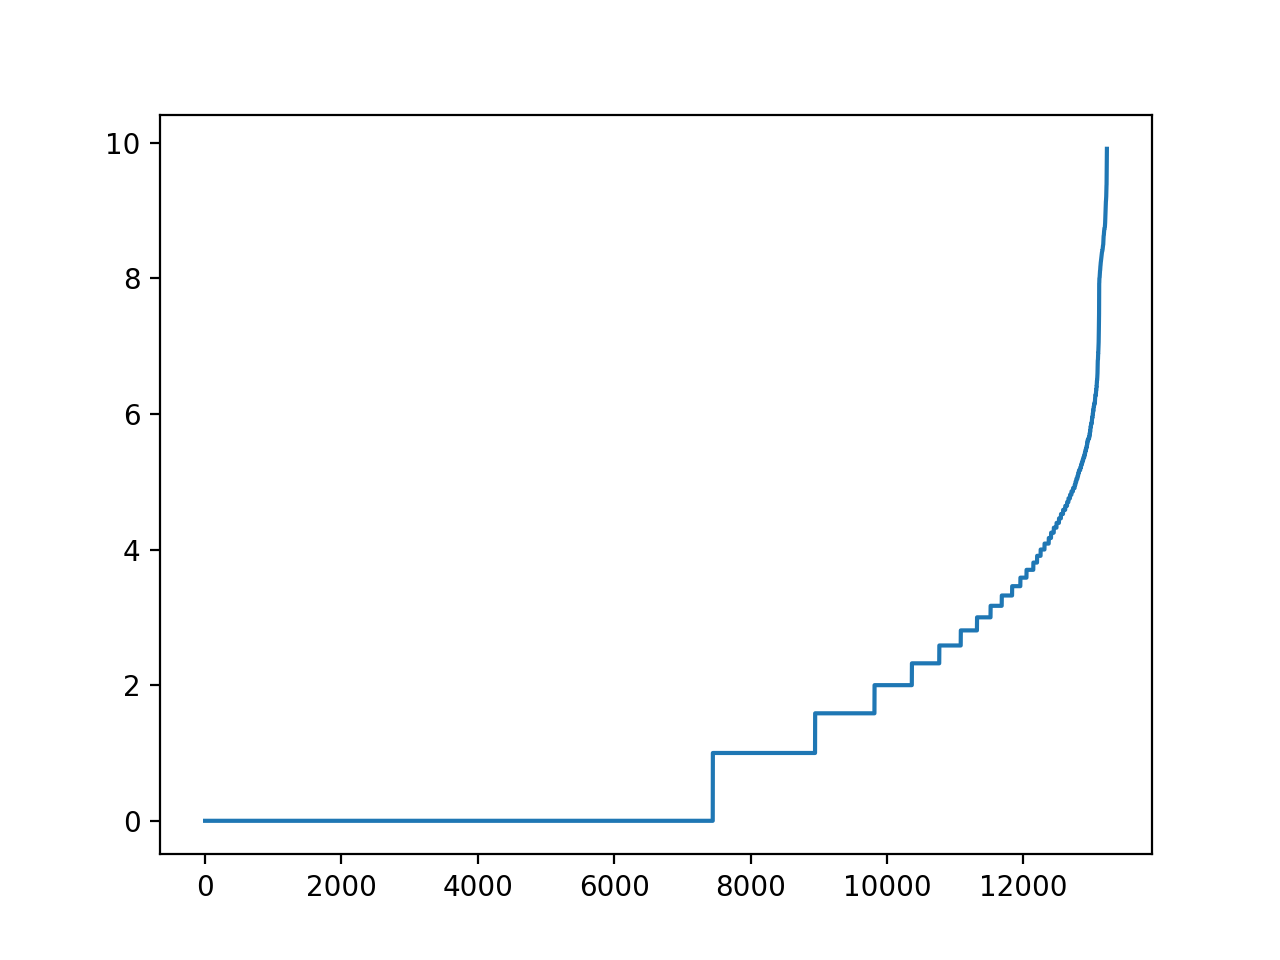
\includegraphics[scale=0.5]{short_path_centrality_ex3_log.png}
        \caption{Rede de jogos de futebol americano.}
        \label{sec5:short_path_centrality_ex3_log}
    \end{subfigure}
    \caption{Distribuição dos valores de centralidade, não normalizados e na escala logarítmica, dos caminhos mínimos.}
    \label{sec5:grafico_centralidade_normalizados}
\end{figure}